\documentclass[11pt]{article}
\usepackage[margin=1in]{geometry}
\usepackage{amsmath}
\usepackage{amssymb}
\usepackage{amsfonts}
\usepackage[round]{natbib}
\usepackage{url}
\usepackage{hyperref}

% Configure hyperref to remove link borders
\hypersetup{
    colorlinks=true,
    linkcolor=black,
    citecolor=black,
    urlcolor=blue,
    pdfborder={0 0 0}
}
\usepackage{graphicx}
\usepackage{array}
\usepackage{booktabs}
\usepackage{xcolor}
\usepackage{soul}
\usepackage{setspace}
\usepackage{subcaption} % For side-by-side figures

\doublespacing

% Set paragraph indentation
\setlength{\parindent}{0.5in}

\title{Bayesian LLM Finetuning for Statistical Inference}
\author{}
\date{}

\begin{document}

\maketitle
\vspace{-1in}

\section{Introduction}

Large language models (LLMs) have increasingly been employed in social science research.
A common workflow involves three stages:
(1) fine-tuning pre-trained LLMs on domain-specific datasets to improve performance on specialized tasks, 
(2) using the fine-tuned models to extract latent variables or classify text data, and 
(3) incorporating these outputs as outcomes or covariates in downstream statistical inference.

However, this approach ignores uncertainty quantification in the LLM output 
estimations, leading to invalid statistical inference. 
As shown in Appendix \ref{appendix:llm_inference}, 
ignoring fine-tuning uncertainty creates four distinct types of inferential problems: 
biased coefficient estimates, invalid standard errors and confidence intervals, 
biased point predictions, and invalid prediction intervals. 

This is especially problematic because fine-tuning on small, 
domain-specific datasets creates systematic overconfidence and measurement errors 
that violate classical assumptions. 
Classical measurement error theory assumes that errors are independent of both the true values being measured and other variables in the analysis, 
leading to predictable attenuation bias that shrinks coefficient estimates toward zero. 
However, fine-tuning-induced measurement errors are systematically correlated with the constructs being measured—for instance, 
when a model trained on imbalanced data consistently overpredicts certain categories. 
Unlike classical measurement error which predictably attenuates coefficients toward zero, 
this bias can be either upward or downward depending on the covariance between fine-tuning-induced measurement errors and the underlying constructs of interest.

Empirical evidence shows that fine-tuned LLMs exhibit overconfidence when adapted to small datasets, 
with parameter-efficient methods like LoRA being particularly susceptible to this issue (Citation: To-be-updated). 
The limited size of typical annotation datasets (often hundreds or thousands of examples) 
relative to the model's billions of parameters creates conditions where models memorize training patterns and
become artificially overconfident about unseen cases (Citation: To-be-updated).

To illustrate the problem, consider a researcher using a fine-tuned LLM to measure political stance 
from social media posts, then using these measures as covariates in a regression predicting voting behavior. 
If the LLM was fine-tuned on a small dataset with predominantly liberal examples, 
it will systematically overpredict liberal stance, 
especially for conservative or ambiguous posts. 
This creates negatively correlated measurement error where errors are 
larger for conservative content, leading to biased coefficient estimates, 
invalid standard errors, and overconfident predictions about voting outcomes.

In this research, we propose a framework that properly accounts for uncertainty 
from LLM fine-tuning in downstream statistical inference. 
Our approach jointly estimates LLM fine-tuning parameters and statistical model parameters 
within a Bayesian framework, rather than the conventional three-stage approach that treats LLM outputs 
as deterministic point estimates. 
Specifically, we obtain posterior distributions over fine-tuning parameters 
using tractable approximations, then propagate this uncertainty to statistical models,
ensuring valid statistical inference. \hl{(We don't have a solution yet)}

A key advantage of our approach is that it enables joint estimation of fine-tuning parameters 
specifically for the downstream statistical task. 
Traditional workflows treat fine-tuning and statistical analysis as separate stages: 
models are first fine-tuned on domain-specific classification or regression tasks, 
then the resulting features are used in entirely different downstream analyses. 
This separation ignores the potential mismatch between the fine-tuning objective 
and the research question. 
Our unified framework allows the fine-tuning process to be jointly optimized with the statistical model, 
enabling the LLM to learn representations that are specifically tailored to the downstream statistical task 
rather than just the intermediate labeling task. 
This joint estimation not only improves predictive performance but also ensures that the uncertainty quantification 
reflects the specific requirements of the statistical analysis, 
leading to more reliable statistical inference for the research question of interest.

\section{Problem Setting}

\subsection{Sources of Uncertainty}

We focus specifically on uncertainty arising from the fine-tuning stage rather than 
the pre-training uncertainty inherent in the base LLM. 
Pre-training uncertainty is essentially unidentifiable without access 
to the massive proprietary training corpus and computational resources, 
while fine-tuning uncertainty is both tractable and often dominates 
when adapting to small domain datasets (Citation: To-be-updated).

Fine-tuning pre-trained LLMs often employs parameter-efficient methods like Low-Rank Adaptation (LoRA) \citep{hu2022lora}. 
Standard LoRA fine-tuning proceeds as follows: 
the pre-trained weights $W_0$ are adapted using low-rank decomposition $W = W_0 + BA$ where $B \in \mathbb{R}^{m \times r}$ and $A \in \mathbb{R}^{r \times n}$ with rank $r \ll \min(m, n)$. 
During fine-tuning, only the LoRA parameters $\theta_{\text{LoRA}} = [A, B]$ 
are optimized on a domain-specific dataset to obtain point estimates $\hat{A}, \hat{B}$.

However, when these methods are applied to domain-specific datasets with limited examples, 
they exhibit pronounced overconfidence issues \citep{yang2023bayesian, wang2024blob}. 
The limited size of typical annotation datasets (often hundreds or thousands of examples) 
relative to the model's billions of parameters creates conditions where models memorize training patterns 
and become artificially overconfident about unseen cases.

This fine-tuning uncertainty is particularly consequential for the downstream statistical inference 
because it violates classical measurement error assumptions. 
Unlike independent measurement errors that lead to attenuation bias, 
fine-tuning errors can be systematically correlated with both the true constructs of interest 
and other variables in the analysis, leading to bias in unpredictable directions.

\subsection{Setup and Notation}

In our framework, observable components are:
(1) raw text data for the downstream statistical task $\{x_i\}_{i=1}^n$, 
(2) structured covariates $Q \in \mathbb{R}^{n \times p}$ and outcome variables $Y \in \mathbb{R}^n$,
(3) a domain-specific fine-tuning dataset $D_{\text{train}} = \{(\tilde{x}_j, \tilde{z}_j)\}_{j=1}^N$ used to adapt the pre-trained LLM, and 
(4) the LoRA parameters $\theta_{\text{LoRA}}$.

The unobservable components include: 
(1) the true latent constructs $z_i$ that we aim to measure from text, 
(2) the massive pre-training dataset and computational resources needed to characterize uncertainty in the base model parameters $W_0$.

The estimable quantities in our framework are: 
(1) approximate posterior distributions over fine-tuning parameters $p(\theta_{\text{LoRA}}|D_{\text{train}})$, 
(2) joint posterior distributions over both LoRA fine-tuning parameters and downstream statistical model parameters, and
(3) posterior predictive distributions that properly account for uncertainty propagation.

\subsection{Bayesian Approach to LoRA Uncertainty}

Standard LoRA fine-tuning treats the fine-tuned parameters as fixed, leading to deterministic feature extraction:
$z_i = f_{\text{LLM}}(x_i; W_0 + \hat{B}\hat{A})$ where $\{x_i\}_{i=1}^n$ is raw text data and $z_i \in \mathbb{R}^d$. However, this approach ignores uncertainty in the fine-tuning parameters, particularly problematic when fine-tuning on small datasets. 

Bayesian fine-tuning \citep{yang2023bayesian, wang2024blob} addresses this by characterizing the full posterior distribution over parameters:
\begin{equation}
p(\theta_{\text{LoRA}}|D_{\text{train}}) \propto p(D_{\text{train}}|\theta_{\text{LoRA}}, W_0)p(\theta_{\text{LoRA}})
\end{equation}
where $p(D_{\text{train}}|\theta_{\text{LoRA}}, W_0)$ is the likelihood of the fine-tuning data and $p(\theta_{\text{LoRA}})$ is the prior over parameters. For feature extraction, instead of deterministic outputs $z_i$, we obtain posterior predictive distributions that integrate over parameter uncertainty:
\begin{equation}
p(z_i|x_i, D_{\text{train}}) = \int p(z_i|x_i, W_0 + \theta_{\text{LoRA}})p(\theta_{\text{LoRA}}|D_{\text{train}})d\theta_{\text{LoRA}}
\end{equation}

This posterior predictive distribution properly reflects uncertainty from the fine-tuning process, providing calibrated feature representations that account for the limited size of domain-specific training data.

\begin{figure}[h]
\centering
\begin{subfigure}[b]{0.48\textwidth}
    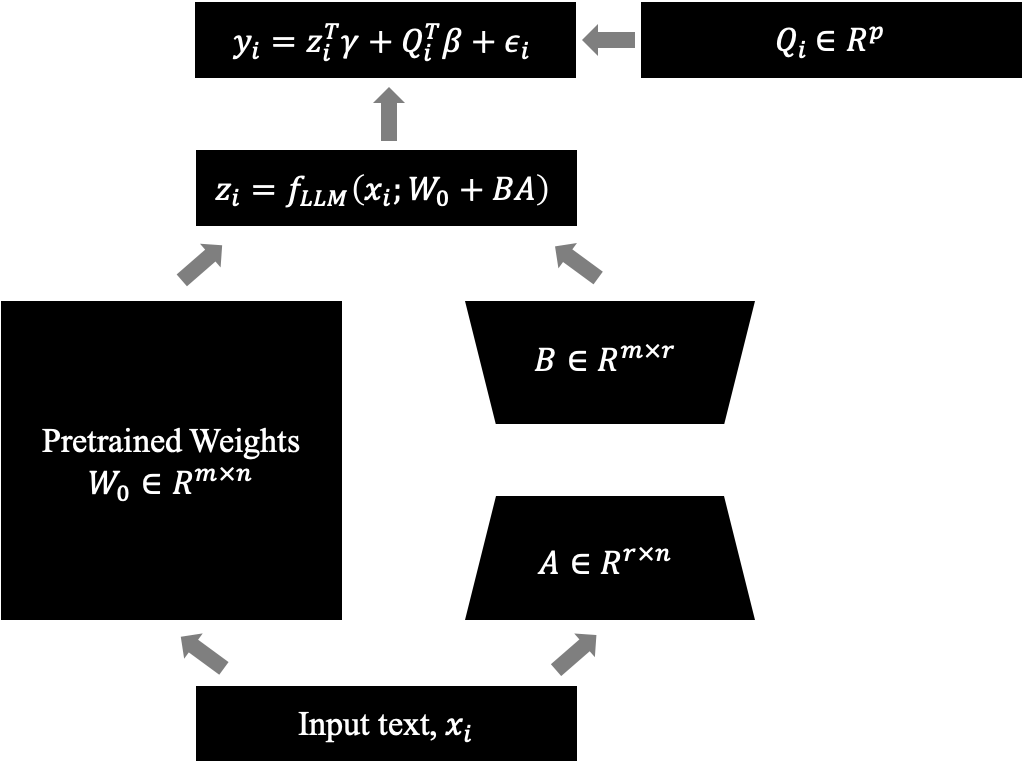
\includegraphics[width=\textwidth]{images/case1_diagram.png}
    \caption{Case A: LLM outputs as covariates}
    \label{fig:case1}
\end{subfigure}
\hfill
\begin{subfigure}[b]{0.48\textwidth}
    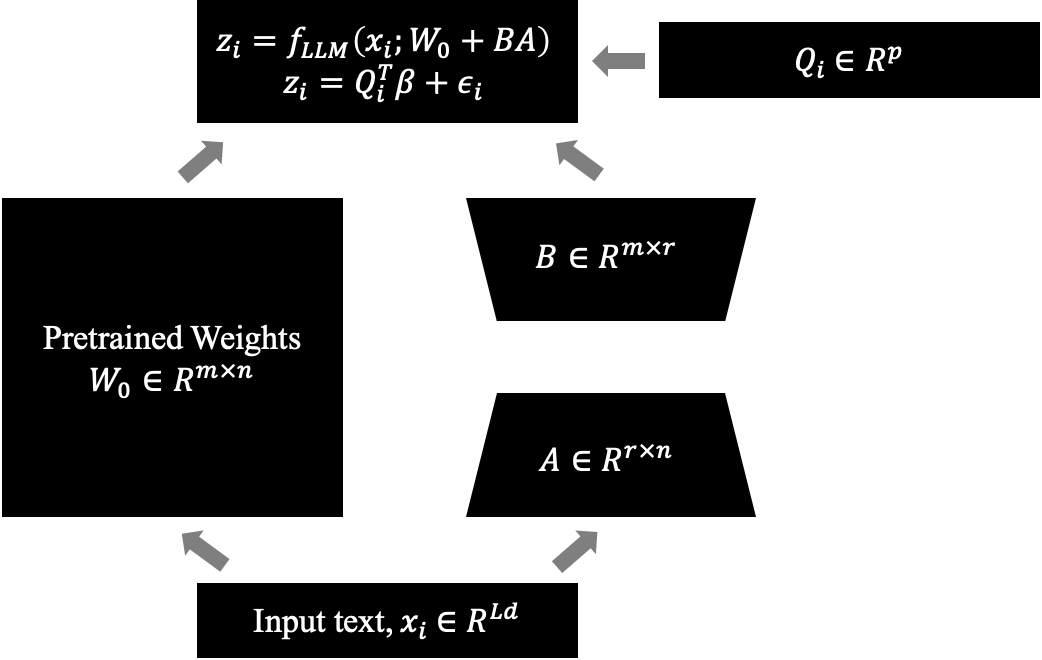
\includegraphics[width=\textwidth]{images/case2_diagram.png}
    \caption{Case B: LLM outputs as outcomes}
    \label{fig:case2}
\end{subfigure}
\caption{Overview of the two cases of LLM uncertainty propagation in statistical inference}
\label{fig:both_cases}
\end{figure}

\subsection{Case A: Inference with LLM Outputs Used as Covariates}

We first consider the case where LLM outputs are used as covariates in downstream statistical models. 
When covariates are measured with error, this leads to attenuation bias—coefficient estimates are biased toward zero—if errors are independent of the input data and can result in underestimating the true effects of LLM-derived variables on outcomes of interest. 
However, this classical measurement error framework does not apply to fine-tuned LLMs, 
where prediction errors systematically depend on the training dataset used for fine-tuning. 
Fine-tuning on small, domain-specific datasets often creates overconfidence issues that lead to systematic prediction biases rather than 
independent measurement errors.
The resulting measurement error violates the independence assumption, 
meaning bias can occur in either direction depending on how the limited training data relates to the broader application domain.

The standard downstream regression with LLM outputs as covariates performs $Y_i = z_i^T\gamma + Q_i^T\beta + \varepsilon_i$, where $Q \in \mathbb{R}^{n \times p}$ represents structured covariates, and $Y \in \mathbb{R}^n$ is an outcome variable. This approach considers $z_i$, LLM outputs, as deterministic data, thus ignoring uncertainty in the LoRA parameters $\theta_{\text{LoRA}}$ from fine-tuning and leading to invalid statistical inference.

We propose a unified Bayesian framework that addresses this by jointly modeling both the feature extraction and statistical modeling stages. Rather than treating $z_i$ as observed covariates, we recognize that $z_i$ are uncertain predictions from a fine-tuned LLM with parameter uncertainty. The joint model specifies:

\begin{align}
\text{Feature extraction:} \quad &p(z_i|x_i, \theta_{\text{LoRA}}, W_0) \label{eq:feature_extraction} \\
\text{Downstream regression model:} \quad &Y_i|z_i, Q_i, \gamma, \beta \sim N(z_i^T\gamma + Q_i^T\beta, \sigma^2) \label{eq:regression_model} \\
\text{LoRA parameter posterior:} \quad &p(\theta_{\text{LoRA}}|D_{\text{train}}) \propto p(D_{\text{train}}|\theta_{\text{LoRA}}, W_0)p(\theta_{\text{LoRA}}) \label{eq:lora_posterior}
\end{align}

The joint inferential target:
\begin{align}
&p(\gamma, \beta, \sigma^2, \theta_{\text{LoRA}}|Y, Q, D_{\text{train}}) \propto \label{eq:joint_target} \\
&\prod_i p(Y_i|z_i, Q_i, \gamma, \beta, \sigma^2)p(z_i|x_i, \theta_{\text{LoRA}}, W_0)p(\theta_{\text{LoRA}}|D_{\text{train}})p(\gamma, \beta, \sigma^2) \nonumber
\end{align}

This joint posterior properly accounts for uncertainty propagation from fine-tuning through to statistical inference, enabling valid statistical inferences that reflect the true uncertainty in LLM-derived measurements.

\subsection{Case B: Inference with LLM outputs Used as Outcomes}

We next consider the alternative case where LLM-generated measures serve as dependent variables in statistical models. Under classical assumptions, where measurement errors are independent of the regressors and mean-zero, errors in the dependent variable do not bias regression coefficients but do inflate the residual variance, leading to larger standard errors and reduced statistical power. However, this classical framework is often violated when LLMs are used as predictive instruments for outcomes. Fine-tuned LLMs, especially those trained on limited or domain-specific data, may exhibit systematic errors that correlate with the input variables or vary in structure across contexts. These violations can introduce endogeneity-like concerns, resulting in biased coefficient estimates and invalid inference. In particular, biased or structured prediction errors from LLMs may confound the relationship between covariates and outcomes, undermining the reliability of statistical conclusions drawn from such models.

The standard approach estimates $z_i = Q_i^T\beta + \varepsilon_i$, where $z_i$ represents the LLM-generated measure of interest and $Q_i$ are explanatory variables. However, researchers observe $\hat{z}_i$ rather than the true construct $z_i$, where $\hat{z}_i$ contains measurement error from the fine-tuning process. This measurement error in the dependent variable contaminates all coefficient estimates $\beta$, and leads to inconsistent standard errors that invalidate hypothesis testing and confidence intervals.

Our unified Bayesian framework addresses this by jointly modeling the statistical relationship and the LLM measurement process. Rather than treating the observed LLM outputs $\hat{z}_i$ as the true dependent variable, our approach recognizes that we observe noisy measurements of an underlying latent construct $z_i$. The joint model specifies:

\begin{align}
\text{Statistical relationship:} \quad &z_i|Q_i, \beta, \sigma^2 \sim N(Q_i^T\beta, \sigma^2) \label{eq:stat_relationship} \\
\text{LLM measurement process:} \quad &\hat{z}_i|x_i, z_i, \theta_{\text{LoRA}} \sim p(\hat{z}_i|x_i, z_i, W_0 + \theta_{\text{LoRA}}) \label{eq:llm_measurement} \\
\text{LoRA parameter posterior:} \quad &p(\theta_{\text{LoRA}}|D_{\text{train}}) \propto p(D_{\text{train}}|\theta_{\text{LoRA}}, W_0)p(\theta_{\text{LoRA}}) \label{eq:lora_posterior2}
\end{align}

The joint inferential target:
\begin{align}
&p(\beta, \sigma^2, Z, \theta_{\text{LoRA}}|\hat{Z}, Q, x_i, D_{\text{train}}) \propto \label{eq:joint_target2} \\
&\prod_i p(z_i|Q_i, \beta, \sigma^2)p(\hat{z}_i|x_i, z_i, \theta_{\text{LoRA}})p(\theta_{\text{LoRA}}|D_{\text{train}})p(\beta, \sigma^2) \nonumber
\end{align}

where $z_i$ are treated as latent variables to be estimated jointly with the regression parameters $\beta$ and LoRA parameters $\theta_{\text{LoRA}}$. This approach enables valid inference about the factors driving the latent construct while properly accounting for both the uncertainty in measuring $z_i$ from text and the parameter uncertainty from fine-tuning.

\newpage
\bibliographystyle{plainnat}
\begin{thebibliography}{99}

\bibitem[Battaglia et~al.(2025)]{battaglia2025inference}
Battaglia, L., Christensen, T., Hansen, S., and Sacher, S. (2025).
\newblock Inference for regression with variables generated by ai or machine learning.

\bibitem[Hu et~al.(2022)]{hu2022lora}
Hu, E.~J., Shen, Y., Wallis, P., Allen-Zhu, Z., Li, Y., Wang, S., Wang, L., and Chen, W. (2022).
\newblock Lora: Low-rank adaptation of large language models.
\newblock {\em ICLR}, 1(2):3.
\newblock \url{https://arxiv.org/abs/2106.09685}

\bibitem[Yang et~al.(2023)]{yang2023bayesian}
Yang, A.~X., Robeyns, M., Wang, X., and Aitchison, L. (2023).
\newblock Bayesian low-rank adaptation for large language models.
\newblock {\em arXiv preprint arXiv:2308.13111}.
\newblock \url{https://arxiv.org/abs/2308.13111}

\bibitem[Wang et~al.(2024)]{wang2024blob}
Wang, Y., Shi, H., Han, L., Metaxas, D., and Wang, H. (2024).
\newblock Blob: Bayesian low-rank adaptation by backpropagation for large language models.
\newblock {\em Advances in Neural Information Processing Systems}, 37:67758--67794.
\newblock \url{https://proceedings.neurips.cc/paper_files/paper/2024/hash/2eebfcf61fdf4fd8ae1aa1c1dbc50066-Abstract-Conference.html}

\bibitem[Zhang et~al.(2023)]{zhang2023debiasing}
Zhang, J., Xue, W., Yu, Y., and Tan, Y. (2023).
\newblock Debiasing ML-or AI-Generated Regressors in Partial Linear Models.
\newblock {\em Available at SSRN 4636026}.
\newblock \url{https://papers.ssrn.com/sol3/papers.cfm?abstract_id=4636026}

\end{thebibliography}

\newpage
\appendix

\section{Consequences of Ignoring LLM Uncertainty Quantification}
\label{appendix:llm_inference}

\subsection{Sources of LLM Uncertainty}
The LLM output uncertainty comes from two sources: (i) baseline uncertainty, reflecting errors inherent in the pre-trained model $f_{\text{LLM}}(x_i; W_0)$, 
and (ii) fine-tuning uncertainty,
reflecting the variability induced by adapting to a small domain-specific dataset.

Let the latent construct of interest (e.g., sentiment, topic proportion, policy position) be denoted by $z_i$. When we apply a pre-trained LLM with parameters $W_0$ to text $x_i$, we obtain an approximation $z_i^{(0)} = f_{\text{LLM}}(x_i; W_0) = z_i + u_i^{(0)}$, where $u_i^{(0)}$ represents baseline error from the pre-trained model. After fine-tuning with LoRA on a small domain dataset $D_{\text{train}}$, we obtain $\tilde{z}_i = f_{\text{LLM}}(x_i; W_0 + \theta_{\text{LoRA}}) = z_i^{(0)} + u_i^{(ft)} = z_i + u_i^{(0)} + u_i^{(ft)}$, where $u_i^{(ft)}$ captures fine-tuning uncertainty.

In principle, both $u_i^{(0)}$ and $u_i^{(ft)}$ contribute to measurement error. However, in this work, we focus on $u_i^{(ft)}$ and consider $u_i^{(0)}$ as absorbed into the latent construct $z_i$. The motivation is twofold: (i) baseline error from pretraining is essentially unidentifiable without access to the massive training corpus, and (ii) fine-tuning error is tractable and often dominates uncertainty when adapting to small domain datasets. By specifying priors on the LoRA parameters, $\theta_{\text{LoRA}}$, and conditioning on the domain-specific dataset $D_{\text{train}}$, its posterior distribution can be approximated, making this error both estimable and consequential for downstream inference.

With this simplification, we write the observed LLM-derived surrogate as $\tilde{z}_i = z_i + u_i$, where $u_i \equiv u_i^{(ft)}$ denotes the fine-tuning error. 
Importantly, $u_i$ may be correlated with the latent construct $z_i$, the structured covariates $Q_i$, and even the regression error $\varepsilon_i$.

This violation of classical measurement error assumptions leads to four distinct types of inferential problems in both cases:
biased coefficient estimates, invalid standard errors and confidence intervals, biased point predictions, and invalid prediction intervals.
We analyze these issues separately for each case below.

\subsection{Inference Issues of Ignoring Fine-Tuning Uncertainty}

\subsubsection{Case A: LLM Outputs as Covariates}

We now show the statistical consequences of ignoring this uncertainty in downstream regression analysis.
Consider the true model follows:
\begin{equation}
Y_i = z_i^T\gamma + Q_i^T\beta + \varepsilon_i, \quad E[\varepsilon_i|z_i, Q_i] = 0
\end{equation}
where $z_i$ represents the latent construct of interest extracted from text $x_i$, $Q_i$ denotes covariates, and $Y_i$ is the outcome variable.
In practice, researchers observe the noisy LLM output $\tilde{z}_i = z_i + u_i$ and
estimate the model using $\tilde{z}_i$ in place of the unobserved true values $z_i$, ignoring the uncertainty in the fine-tuning process.

To analyze the bias introduced by this substitution, we employ the residual maker $M_Q = I - Q(Q'Q)^{-1}Q'$ to partial out the covariates. 
Let $\dot{z} = M_Q\tilde{z}$, $z^* = M_Q z$, $\dot{u} = M_Q u$, and $\dot{\varepsilon} = M_Q \varepsilon$ denote the variables after partialling out $Q$. The OLS estimator for $\gamma$ becomes:
\begin{equation}
\hat{\gamma} = (\dot{z}'\dot{z})^{-1}\dot{z}'\dot{Y}
\end{equation}
where $\dot{Y} = \gamma z^* + \dot{\varepsilon}$ represents the true model after transformation.

Substituting the relationship $\dot{z} = z^* + \dot{u}$ into the OLS formula yields:
\begin{equation}
\hat{\gamma} = \frac{(z^* + \dot{u})'(\gamma z^* + \dot{\varepsilon})}{(z^* + \dot{u})'(z^* + \dot{u})}
\end{equation}

The numerator expands to $\gamma (z^*)' z^* + (z^*)' \dot{\varepsilon} + \gamma \dot{u}' z^* + \dot{u}' \dot{\varepsilon}$, while the denominator becomes $(z^*)' z^* + 2(z^*)' \dot{u} + \dot{u}' \dot{u}$. Taking probability limits and applying the exogeneity assumption $\text{Cov}(z^*, \dot{\varepsilon}) = 0$, we obtain:
\begin{equation}
\text{plim } \hat{\gamma} = \gamma \cdot \frac{\text{Var}(z^*) + \text{Cov}(z^*, \dot{u})}{\text{Var}(z^*) + \text{Var}(\dot{u}) + 2\text{Cov}(z^*, \dot{u})} + \frac{\text{Cov}(\dot{u}, \dot{\varepsilon})}{\text{Var}(\dot{z})} \tag{A1}
\end{equation}

This result reveals several important deviations from classical measurement error, with consequences for both estimation and inference.

\textbf{Biased coefficient estimates:} The classical measurement error assumes $u \perp (z, Q, \varepsilon)$ with $E[u] = 0$,
yielding the attenuation bias:
\begin{equation}
\text{plim } \hat{\gamma} = \gamma \cdot \frac{\text{Var}(z^*)}{\text{Var}(z^*) + \text{Var}(\dot{u})} \in (0,1) \cdot \gamma \quad \text{(attenuation)} \tag{A2}
\end{equation}

However, this classical case rarely applies to fine-tuned LLMs due to two key violations. 
Structured measurement error occurs when $\text{Cov}(z^*, \dot{u}) \neq 0$—arising from overconfident 
patterns learned from small training datasets—causing the bias in equation (A1) to be either upward or downward. 
Endogeneity-type correlation emerges when LLM errors correlate with the regression error ($\text{Cov}(\dot{u}, \dot{\varepsilon}) \neq 0$), 
where the second term in equation (A1) introduces additional bias that compounds the measurement error problem.

\textbf{Invalid standard errors and confidence intervals:} Standard OLS procedures treat $\dot{z}$ as fixed regressors and construct confidence intervals 
around the pseudo-true limit in equation (A1) rather than the true parameter $\gamma$. 
This creates two distinct problems: (1) confidence intervals center around the biased probability limit from equation (A1)
rather than the true parameter $\gamma$, leading to systematic mis-coverage; and (2) variance underestimation,
where the variance calculations omit first-stage uncertainty from LLM fine-tuning.

\textbf{Biased point predictions:} Plug-in predictions $\hat{Y}_i = \hat{\gamma} \tilde{z}_i + Q_i'\hat{\beta}$ 
suffer from two sources of bias: coefficient bias, where predictions inherit the bias in $\hat{\gamma}$ from equation (A1),
and input bias, where the systematic distortion in $\tilde{z}_i$
(using noisy LLM outputs instead of true values) further distorts predictions. 
The combined effect yields systematically biased mean predictions, with the direction (upward or downward bias)
depending on the sign of the bias in equation (A1).

\textbf{Invalid prediction intervals:} 
Standard prediction intervals ignore LLM uncertainty and use only the residual variance $\sigma^2$. 
However, the correct conditional predictive variance includes additional uncertainty terms. 
Starting from the true model $Y_i = \gamma z_i + Q_i'\beta + \varepsilon_i$ and substituting $z_i = \tilde{z}_i - u_i$, 
we get $Y_i = \gamma\tilde{z}_i + Q_i'\beta - \gamma u_i + \varepsilon_i$. The conditional variance becomes:
\begin{equation}
\text{Var}(Y_i | Q_i, \tilde{z}_i) = \sigma^2 + \gamma^2\text{Var}(u_i | x_i, D_{\text{train}}) + 2\gamma \text{Cov}(u_i, \varepsilon_i | Q_i, \tilde{z}_i) \tag{A3}
\end{equation}
where we use $\text{Var}(u_i | x_i, D_{\text{train}})$ because LLM measurement error depends on the text input and fine-tuning dataset rather than the covariates. 
The three components represent: the usual regression error variance ($\sigma^2$), 
additional uncertainty from LLM measurement error ($\gamma^2\text{Var}(u_i | x_i, D_{\text{train}})$), 
and cross-correlation between measurement error and regression error ($2\gamma \text{Cov}(u_i, \varepsilon_i)$). 
Omitting these components produces prediction intervals that are systematically too narrow, 
leading to overconfident predictions about future outcomes.

\subsubsection{Case B: LLM Outputs as Outcomes}  

Consider next the case where LLM-derived measures serve as dependent variables. The latent structural relationship is:
\begin{equation}
z_i = Q_i'\beta + \varepsilon_i, \quad E[\varepsilon_i | Q_i] = 0
\end{equation}
where researchers observe $\hat{z}_i = z_i + u_i$ and estimate the model by regressing $\hat{z}_i$ on $Q_i$. The resulting OLS estimator satisfies:
\begin{equation}
\hat{\beta} = \beta + (Q'Q)^{-1}Q'u
\end{equation}
which converges in probability to:
\begin{equation}
\text{plim } \hat{\beta} = \beta + (E[Q_i Q_i'])^{-1} E[Q_i u_i] \tag{B1}
\end{equation}

\textbf{Biased coefficient estimates.} This expression reveals that coefficient bias depends entirely on whether fine-tuning errors correlate with the covariates. When $E[Q_i u_i] \neq 0$—for instance, when fine-tuning errors systematically depend on observable features correlated with $Q_i$—the estimator becomes biased according to equation (B1). For a single regressor, this simplifies to:
\begin{equation}
\text{plim } \hat{\beta} = \beta + \frac{\text{Cov}(Q, u)}{\text{Var}(Q)} \tag{B2}
\end{equation}

\textbf{Invalid standard errors and confidence intervals.} Even when coefficient estimates remain unbiased ($E[Q_i u_i] = 0$), 
the regression errors become $\varepsilon_i + u_i$ because we observe $\hat{z}_i = z_i + u_i$ instead of the true $z_i$, 
so the LLM measurement error $u_i$ appears as additional noise in the residuals alongside the structural error $\varepsilon_i$. 
This creates two opposing effects on confidence intervals: the observed residual variance 
inflates to $\text{Var}(\varepsilon_i + u_i) = \text{Var}(\varepsilon_i) + \text{Var}(u_i) + 2\text{Cov}(\varepsilon_i, u_i)$ (making intervals wider), 
while standard error calculations treat $\hat{z}_i$ as fixed data rather than estimates with uncertainty,
omitting the additional variance component $\text{Var}(\hat{\beta} | \hat{z})$ that accounts for first-stage estimation (making intervals narrower). 
The net effect on coverage depends on whether $\text{Var}(u_i) + 2\text{Cov}(\varepsilon_i, u_i)$ outweighs the ignored first-stage uncertainty,
but likely results in invalid inference due to centering around the wrong target and incorrect variance estimation.

\textbf{Biased predictions.} When $\text{Cov}(Q_i, u_i) \neq 0$, the coefficient estimates are biased according to equation (B1), 
so predictions of the true latent construct are systematically biased: $E[\hat{z}_j | Q_j] - E[z_j | Q_j] = Q_j'(E[Q_i Q_i'])^{-1} E[Q_i u_i]$, 
where the magnitude and direction of bias depend on both the covariate values $Q_j$ and the correlation structure between LLM errors and covariates.

\textbf{Invalid prediction intervals.} Standard procedures use the residual variance 
$\text{Var}(\varepsilon_i + u_i) = \text{Var}(\varepsilon_i) + \text{Var}(u_i) + 2\text{Cov}(\varepsilon_i, u_i)$ 
rather than the true latent variance $\text{Var}(\varepsilon_i)$, producing prediction intervals 
for the latent construct $z_i$ that overestimate uncertainty when $\text{Cov}(\varepsilon_i, u_i) = 0$ due 
to the additional measurement error variance $\text{Var}(u_i)$.

\subsection{Empirical Examples of Fine-Tuning Bias}

For example, suppose $z_i$ is the true stance of a political text, 
and the fine-tuned LLM was trained on a small, imbalanced dataset with mostly liberal examples. 
A researcher then uses these LLM-predicted stance measures as covariates in a regression predicting voting behavior ($Y_i$), 
such as whether individuals vote for conservative candidates. 
The fine-tuned model tends to systematically over-predict liberal stance, 
especially for borderline cases. In this case, the fine-tuning error $u_i$ is larger (and systematically biased) 
when $z_i$ is conservative, $\text{Cov}(u_i, z_i) \neq 0$. 
Similarly, if a structured covariate $Q_i$ captures demographic attributes (e.g., age or region) that affect writing style, 
fine-tuning errors may be larger for certain groups, leading to $\text{Cov}(u_i, Q_i) \neq 0$. 
Finally, if the same unobserved factors affect both the downstream regression and misclassification by the LLM, 
then $\text{Cov}(u_i, \varepsilon_i) \neq 0$. 
These violate the independence assumptions of classical measurement error, 
causing bias that can amplify rather than attenuate coefficient estimates.

\end{document}